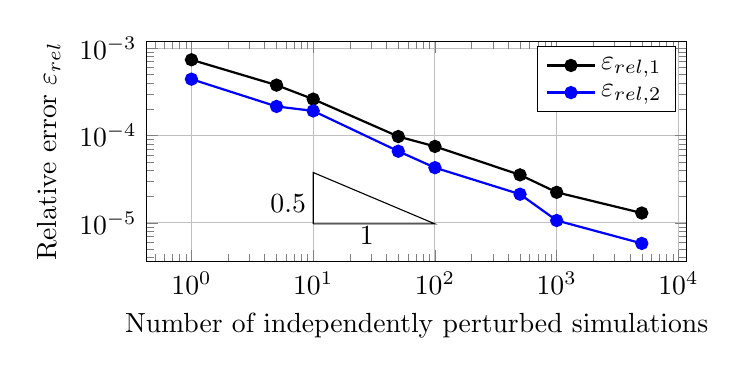
\begin{tikzpicture}
		\centering
		\begin{axis}[scale=0.8,grid=major,
		             width=4in,
		             height=2in,
		             xmode=log,
		             ymode=log,
		             xlabel={Number of independently perturbed simulations},
		             ylabel={Relative error $\varepsilon_{\text{rel}}$}]


	    \addplot[mark=*, mark options={solid}, thick, black] 
	  table[row sep=crcr]{%
   1.000000000000000000e+00 7.365351520800415613e-04\\
5.000000000000000000e+00 3.774890516199529990e-04\\
1.000000000000000000e+01 2.609794287904584854e-04\\
5.000000000000000000e+01 9.740666956990822129e-05\\
1.000000000000000000e+02 7.507652967076603931e-05\\
5.000000000000000000e+02 3.546027706560411162e-05\\
1.000000000000000000e+03 2.239143273328837372e-05\\
5.000000000000000000e+03 1.297876602647626835e-05\\
};
    \addlegendentry{$\varepsilon_{\text{rel},1}$}
        \addplot[mark=*, mark options={solid}, thick, blue] 
	  table[row sep=crcr]{%
   1.000000000000000000e+00 4.418584099850594079e-04\\
5.000000000000000000e+00 2.152931302736786178e-04\\
1.000000000000000000e+01 1.913457767349561578e-04\\
5.000000000000000000e+01 6.613990716869041218e-05\\
1.000000000000000000e+02 4.288601696995630603e-05\\
5.000000000000000000e+02 2.129573824863525007e-05\\
1.000000000000000000e+03 1.065747171006640495e-05\\
5.000000000000000000e+03 5.824285123109026488e-06\\
   };
    \addlegendentry{$\varepsilon_{\text{rel},2}$}

    %\addplot[mark=none] coordinates {(1, 9.74e-06) (5, 9.74e-06) (1, 2.61e-05) (1, 9.74e-06)};
    \addplot[mark=none] coordinates {(10, 9.74e-06) (100, 9.74e-06) (10, 3.775e-05) (10, 9.74e-06)};
		\end{axis}
	\draw[](2.8, 0.09) node[above, text=black]{1};
	\draw[](1.8, 0.5) node[above, text=black]{0.5};
	\end{tikzpicture}